\documentclass[11pt,a4paper]{report}
\usepackage[utf8]{inputenc}
\usepackage[T1]{fontenc}
\usepackage[indonesian]{babel}
\usepackage{amsmath,amsfonts,amssymb,amsthm}
\usepackage{geometry}
\geometry{margin=1in, headheight=14pt}
\usepackage{xcolor}
\usepackage{booktabs}
\usepackage{longtable}
\usepackage{array}
\usepackage{enumitem}
\usepackage{graphicx}
\usepackage{float}
\usepackage{fancyhdr}
\usepackage{tcolorbox}
\tcbuselibrary{skins,breakable}
\usepackage{listings}
\usepackage{tikz}
\usetikzlibrary{shapes,arrows.meta,positioning}
\usepackage{hyperref}

% --- Skema Warna Khas UNIB / Optimisasi ---
\definecolor{unibblue}{RGB}{0,51,102}
\definecolor{unibgold}{RGB}{212,175,55}
\definecolor{unibgreen}{RGB}{0,128,0}
\definecolor{unibred}{RGB}{165,28,48}
\definecolor{codebg}{RGB}{246,248,251}

\hypersetup{
  colorlinks=true,
  linkcolor=unibblue,
  urlcolor=unibblue,
  citecolor=unibgreen,
  pdftitle={Analisis Aliran Daya Menggunakan Python},
  pdfauthor={Novalio Daratha}
}

% --- Header & Footer (Gaya Optimisasi / UNIB) ---
\pagestyle{fancy}
\fancyhf{}
\fancyhead[L]{\small\color{gray}\textit{Analisis Aliran Daya Menggunakan Python}}
\fancyhead[R]{\small\color{gray}\leftmark}
\fancyfoot[L]{\small Universitas Bengkulu - Teknik Elektro}
\fancyfoot[R]{\small\thepage}
\renewcommand{\headrulewidth}{0.4pt}
\renewcommand{\footrulewidth}{0.4pt}
\renewcommand{\footrule}{{\color{gray}\hrule width\headwidth height\footrulewidth \vskip 2pt}}

\fancypagestyle{plain}{
  \fancyhf{}
  \fancyfoot[L]{\small Universitas Bengkulu - Teknik Elektro}
  \fancyfoot[R]{\small\thepage}
  \renewcommand{\headrulewidth}{0pt}
  \renewcommand{\footrulewidth}{0.4pt}
  \renewcommand{\footrule}{{\color{gray}\hrule width\headwidth height\footrulewidth \vskip 2pt}}
}

% --- Kotak Estetis tcolorbox ---
\newtcolorbox{checkpointbox}[1][Titik Periksa Mandiri]{
  colback=unibgreen!6,
  colframe=unibgreen!80!black,
  fonttitle=\bfseries,
  title={#1},
  breakable,
  arc=3pt
}

\newtcolorbox{catatanbox}[1][Catatan Rekayasa]{
  colback=unibblue!6,
  colframe=unibblue!85!black,
  fonttitle=\bfseries,
  title={#1},
  breakable,
  arc=3pt
}

\newtcolorbox{peringatanbox}[1][Perhatian Konvensi]{
  colback=unibgold!14,
  colframe=unibgold!80!black,
  coltitle=black,
  fonttitle=\bfseries,
  title={#1},
  breakable,
  arc=3pt
}

% --- Gaya Listing Python ---
\lstset{
  language=Python,
  basicstyle=\ttfamily\footnotesize,
  backgroundcolor=\color{codebg},
  frame=single,
  rulecolor=\color{unibblue!35},
  keywordstyle=\color{unibblue}\bfseries,
  commentstyle=\color{unibgreen!75!black}\itshape,
  stringstyle=\color{unibred},
  numbers=left,
  numberstyle=\tiny\color{gray},
  stepnumber=1,
  numbersep=8pt,
  showstringspaces=false,
  breaklines=true,
  tabsize=4
}

\begin{document}

% ==================== HALAMAN SAMPUL ====================
\begin{titlepage}
  \centering
  \vspace*{0.8cm}
  {\color{unibblue}\rule{\textwidth}{2.5pt}}\\[0.4cm]
  {\large\bfseries\color{unibblue} BUKU AJAR \& PANDUAN PELATIHAN TEKNIS INTENSIF}\\[0.25cm]
  {\color{unibgold}\rule{0.45\textwidth}{1.5pt}}\\[1.3cm]

  {\Huge\bfseries\color{unibblue} Analisis Aliran Daya\\(Power Flow Analysis)\\Menggunakan Python\par}
  \vspace{0.6cm}
  {\Large\itshape Dari Algoritma Numerik From-Scratch hingga Aplikasi Industri,\\Kontinjensi $N-1$, dan Seri Lanjutan Level 2 (AC-OPF, PV Hosting \& Risiko $N-2$)\par}
  \vspace{1.4cm}

  \begin{tikzpicture}[
    node distance=0.45cm,
    b/.style={draw=unibblue, fill=unibblue!8, rounded corners=4pt, minimum width=2.7cm, minimum height=1.05cm, align=center, font=\footnotesize\bfseries},
    arr/.style={-{Stealth[length=2.4mm]}, thick, color=unibblue}
  ]
    \node[b] (m1) {Modul 1\\$Y_{\text{bus}}$ Sparse};
    \node[b, right=of m1] (m2) {Modul 2\\NR, FDLF \& GS};
    \node[b, right=of m2] (m3) {Modul 3\\\texttt{pandapower}};
    \node[b, right=of m3] (m4) {Modul 4\\Kontinjensi $N-1$};
    \node[b, below=0.8cm of m2, xshift=1.55cm, minimum width=8.2cm, fill=unibgold!20, draw=unibgold!80!black] (l2) {Seri Lanjutan Level 2: AC-OPF (LMP) $\bullet$ PV Hosting Capacity $\bullet$ Risiko $N-2$};
    \draw[arr] (m1) -- (m2);
    \draw[arr] (m2) -- (m3);
    \draw[arr] (m3) -- (m4);
    \draw[arr] (m4.south) |- (l2.east);
  \end{tikzpicture}

  \vfill
  {\large\bfseries Novalio Daratha}\\[0.2cm]
  Program Studi Teknik Elektro, Fakultas Teknik\\
  Universitas Bengkulu\\[0.4cm]
  Portal Interaktif: \url{https://ndaratha.my.id/w-pf/}\\[0.3cm]
  {\small Edisi 1.0 --- November 2026}
\end{titlepage}

\tableofcontents
\newpage

% ==================== BAB 1: PENDAHULUAN ====================
\chapter{Pendahuluan \& Peta Kurikulum}

\section{Latar Belakang Pedagogis}
Analisis aliran daya (\textit{load flow / power flow}) merupakan tulang punggung perhitungan dalam operasi dan perencanaan sistem tenaga listrik. Hampir seluruh studi lanjutan---mulai dari analisis kontinjensi, \textit{optimal power flow} (OPF), stabilitas dinamik, hingga kajian \textit{hosting capacity} energi terbarukan---selalu bertumpu pada satu solusi aliran daya yang akurat.

Buku ajar dan panduan pelatihan ini menjembatani kesenjangan antara teori numerik dan perangkat industri. Pada \textbf{Level 1 (32 JP / 4 Hari)}, peserta terlebih dahulu membangun \textit{solver} aliran daya secara \textit{white-box} menggunakan NumPy dan SciPy Sparse (\texttt{ybus.py} dan \texttt{newton\_raphson.py}), memvalidasi hasilnya hingga presisi mesin ($4{,}44\times 10^{-16}\text{ p.u.}$) terhadap \texttt{pandapower}, lalu mengotomatisasi skrining keamanan kontinjensi $N-1$ (\texttt{pandapower\_workflow.py}). Selanjutnya, \textbf{Bab 6} memperkenalkan \textbf{Seri Lanjutan Level 2 (24 JP / 3 Hari)} yang mencakup AC-OPF, \textit{PV Hosting Capacity}, dan skrining kontinjensi ganda $N-2$ berbasis risiko.

\section{Prasyarat \& Jadwal Pelatihan Level 1 (32 JP)}

\begin{table}[H]
\centering
\caption{Jadwal Pelatihan Intensif Level 1 (4 Hari $\times$ 8 Jam = 32 Jam Pelatihan)}
\small
\begin{tabular}{@{}clll@{}}
\toprule
\textbf{Hari} & \textbf{Sesi Pagi (08.30--12.00)} & \textbf{Sesi Siang (13.00--16.30)} & \textbf{Luaran Terukur} \\
\midrule
1 & Modul 1: Per-unit, model $\pi$ \& trafo & Lab 1: \texttt{build\_ybus()} sparse CSR & Fungsi $Y_{\text{bus}}$ tervalidasi \\
2 & Modul 2: NR polar, Jacobian, $Q$-limit & Lab 2: Solver NR, FDLF-XB \& GS & Solver \& kurva konvergensi \\
3 & Modul 3: Model data \texttt{pandapower} & Lab 3: IEEE 14/30-Bus, profil $V$ & Laporan audit neraca daya \\
4 & Modul 4: Kriteria $N-1$ \& indeks $PI$ & Lab 4 + Presentasi Capstone & Dashboard kontinjensi $N-1$ \\
\bottomrule
\end{tabular}
\end{table}

\begin{catatanbox}[Konvensi Notasi Utama]
Semua besaran dinyatakan dalam per-unit dengan daya dasar $S_{\text{base}} = 100\text{ MVA}$ kecuali disebut lain: $N_b$ jumlah bus, $N_l$ jumlah cabang, $V_i = |V_i|\angle\theta_i$ fasor tegangan bus $i$, $Y_{ik} = G_{ik} + jB_{ik}$ elemen matriks admitansi bus, $\theta_{ik} = \theta_i - \theta_k$, dan $S_i = P_i + jQ_i$ injeksi daya bersih ke bus $i$ (pembangkitan dikurangi beban).
\end{catatanbox}

% ==================== BAB 2: MODUL 1 ====================
\chapter{Modul 1: Pemodelan Jaringan \& Matriks Admitansi Bus ($Y_{\text{bus}}$)}

\section{Tujuan Pembelajaran (Taksonomi Bloom C1--C5)}
\begin{itemize}[leftmargin=1.5em]
  \item \textbf{[C1--C2]} Mengklasifikasikan bus \textit{Slack}, \textit{PV}, dan \textit{PQ} serta menjelaskan model nominal-$\pi$ dan trafo \textit{off-nominal tap / phase-shifter}.
  \item \textbf{[C3]} Menerapkan sistem per-unit dan membangun fungsi \texttt{build\_ybus()} berbasis \texttt{scipy.sparse.csr\_matrix}.
  \item \textbf{[C4--C5]} Menganalisis sifat sparsitas, simetri, serta memvalidasi $Y_{\text{bus}}$ terhadap pustaka referensi.
\end{itemize}

\section{Ringkasan Teori \& Persamaan Utama}

\subsection{Sistem Per-Unit \& Klasifikasi Bus}
\begin{equation}
  Z_{\text{base}} = \frac{V_{\text{base,LL}}^2}{S_{\text{base}}}, \qquad
  z_{\text{pu}} = \frac{Z_{\Omega}}{Z_{\text{base}}}, \qquad
  z_{\text{pu}}^{\text{baru}} = z_{\text{pu}}^{\text{lama}}\left(\frac{V_{\text{base}}^{\text{lama}}}{V_{\text{base}}^{\text{baru}}}\right)^2\frac{S_{\text{base}}^{\text{baru}}}{S_{\text{base}}^{\text{lama}}}
\end{equation}

\begin{table}[H]
\centering
\caption{Klasifikasi Tipe Bus dalam Studi Aliran Daya}
\small
\begin{tabular}{@{}llll@{}}
\toprule
\textbf{Jenis Bus} & \textbf{Diketahui} & \textbf{Dicari} & \textbf{Peran Fisik} \\
\midrule
Slack / Referensi (REF) & $|V|,\; \theta = 0$ & $P,\; Q$ & Menutup neraca daya \& rugi; referensi sudut \\
Generator (PV) & $P,\; |V|$ & $Q,\; \theta$ & Generator dengan AVR ($Q_{\min} \le Q \le Q_{\max}$) \\
Beban (PQ) & $P,\; Q$ & $|V|,\; \theta$ & Beban daya konstan atau PV terkunci batas $Q$ \\
\bottomrule
\end{tabular}
\end{table}

\subsection{Model Umum Cabang Nominal-$\pi$ \& Trafo Kompleks}
Untuk cabang ke-$l$ antara bus pengirim $f$ dan penerima $t$ dengan admitansi seri $y_s = (R + jX)^{-1}$, suseptansi \textit{charging} total $B$, serta rasio tap kompleks $a = t\,e^{j\varphi}$ di sisi $f$:
\begin{equation}
  \begin{bmatrix} I_f \\ I_t \end{bmatrix} =
  \begin{bmatrix}
    \dfrac{y_s + j\frac{B}{2}}{|a|^2} & -\dfrac{y_s}{a^*} \\[10pt]
    -\dfrac{y_s}{a} & y_s + j\frac{B}{2}
  \end{bmatrix}
  \begin{bmatrix} V_f \\ V_t \end{bmatrix}
  =
  \begin{bmatrix} Y_{ff} & Y_{ft} \\ Y_{tf} & Y_{tt} \end{bmatrix}
  \begin{bmatrix} V_f \\ V_t \end{bmatrix}
\end{equation}
Menggunakan matriks insidensi cabang $C_f, C_t \in \{0,1\}^{N_l \times N_b}$ dan admitansi shunt bus $Y_{\text{sh},i} = (G_{S,i} + jB_{S,i})/S_{\text{base}}$:
\begin{align}
  Y_f &= \operatorname{diag}(Y_{ff}) C_f + \operatorname{diag}(Y_{ft}) C_t, \qquad
  Y_t = \operatorname{diag}(Y_{tf}) C_f + \operatorname{diag}(Y_{tt}) C_t \\
  Y_{\text{bus}} &= C_f^{\mathsf{T}} Y_f + C_t^{\mathsf{T}} Y_t + \operatorname{diag}(Y_{\text{sh}})
\end{align}

\section{Tugas Lab, Titik Periksa \& Rubrik Modul 1}
Peserta membangun fungsi \texttt{build\_ybus()} sparse pada \texttt{ybus.py}, menguji pemetaan nomor bus eksternal tak-berurutan, serta memvisualisasikan pola sparsitas.

\begin{checkpointbox}[Titik Periksa Mandiri Modul 1 (IEEE 14-Bus)]
\begin{itemize}[leftmargin=1.3em]
  \item Dimensi $Y_{\text{bus}}$: $14 \times 14$ dengan \texttt{nnz} = \textbf{54} (sparsitas $72{,}45\%$, densitas $27{,}55\%$).
  \item Elemen diagonal Slack Bus 1: $Y_{11} = \mathbf{6{,}0250 - j19{,}4471\text{ p.u.}}$
  \item Norma asimetri tanpa \textit{phase-shifter}: $\|Y_{\text{bus}} - Y_{\text{bus}}^{\mathsf{T}}\|_{\infty} = \mathbf{0{,}0}$.
\end{itemize}
\end{checkpointbox}

% ==================== BAB 3: MODUL 2 ====================
\chapter{Modul 2: Algoritma Numerik Aliran Daya \textit{From-Scratch}}

\section{Formulasi Polar Newton-Raphson \& Matriks Jacobian}
Injeksi daya aktif dan reaktif terhitung pada bus $i$ adalah:
\begin{align}
  P_i(\boldsymbol{\theta}, |\mathbf{V}|) &= |V_i|\sum_{k=1}^{N_b} |V_k|\left(G_{ik}\cos\theta_{ik} + B_{ik}\sin\theta_{ik}\right) \\
  Q_i(\boldsymbol{\theta}, |\mathbf{V}|) &= |V_i|\sum_{k=1}^{N_b} |V_k|\left(G_{ik}\sin\theta_{ik} - B_{ik}\cos\theta_{ik}\right)
\end{align}
Dengan vektor koreksi $\Delta\mathbf{x} = [\Delta\boldsymbol{\theta}_{\mathcal{PV}\cup\mathcal{PQ}};\; \Delta|\mathbf{V}|_{\mathcal{PQ}}]^{\mathsf{T}}$ berdimensi $n = N_{\text{PV}} + 2N_{\text{PQ}}$ ($n = 22$ pada IEEE 14-Bus), sistem linier Newton-Raphson diselesaikan dengan \texttt{scipy.sparse.linalg.spsolve}:
\begin{equation}
  \begin{bmatrix} \mathbf{H} & \mathbf{N} \\ \mathbf{M} & \mathbf{L} \end{bmatrix}
  \begin{bmatrix} \Delta\boldsymbol{\theta} \\ \Delta|\mathbf{V}| \end{bmatrix}
  =
  \begin{bmatrix} \Delta\mathbf{P} \\ \Delta\mathbf{Q} \end{bmatrix}
\end{equation}

\begin{table}[H]
\centering
\caption{Rumus Eksplisit Empat Sub-Matriks Jacobian Polar ($J_1, J_2, J_3, J_4$)}
\small
\begin{tabular}{@{}lll@{}}
\toprule
\textbf{Sub-Matriks} & \textbf{Off-Diagonal ($i \neq k$)} & \textbf{Diagonal ($i = k$)} \\
\midrule
$H_{ik} = \partial P_i/\partial\theta_k$ & $|V_i||V_k|(G_{ik}\sin\theta_{ik} - B_{ik}\cos\theta_{ik})$ & $-Q_i - B_{ii}|V_i|^2$ \\
$N_{ik} = \partial P_i/\partial|V_k|$ & $|V_i|(G_{ik}\cos\theta_{ik} + B_{ik}\sin\theta_{ik})$ & $P_i/|V_i| + G_{ii}|V_i|$ \\
$M_{ik} = \partial Q_i/\partial\theta_k$ & $-|V_i||V_k|(G_{ik}\cos\theta_{ik} + B_{ik}\sin\theta_{ik})$ & $P_i - G_{ii}|V_i|^2$ \\
$L_{ik} = \partial Q_i/\partial|V_k|$ & $|V_i|(G_{ik}\sin\theta_{ik} - B_{ik}\cos\theta_{ik})$ & $Q_i/|V_i| - B_{ii}|V_i|$ \\
\bottomrule
\end{tabular}
\end{table}

\section{Penegakan Batas Daya Reaktif ($Q$-Limit) \& Perbandingan Solver}
Implementasi \texttt{newton\_raphson.py} menegakkan batas $Q_{\min} \le Q_{G,i} \le Q_{\max}$ dengan agregasi multi-generator per bus (\texttt{np.add.at}), seleksi pelanggaran terbesar per siklus (\textit{largest-violation-first}), serta \textit{back-switching} $PQ \to PV$ berdasarkan syarat komplementaritas AVR.

\begin{figure}[H]
  \centering
  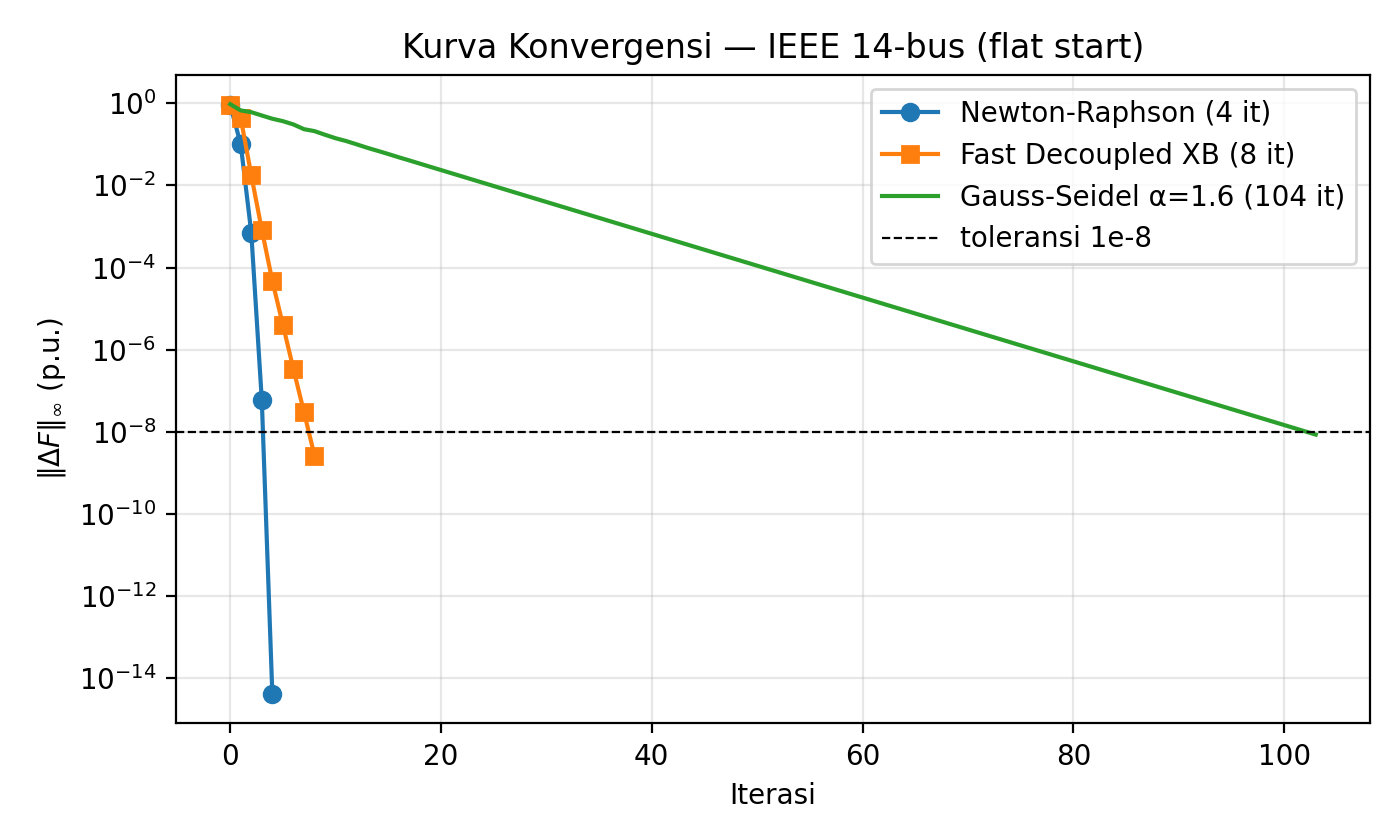
\includegraphics[width=0.82\textwidth]{../figures/konvergensi.png}
  \caption{Perbandingan kurva konvergensi Newton-Raphson (4 iterasi), FDLF-XB (8 iterasi), dan Gauss-Seidel terakselerasi $\alpha=1{,}6$ (104 iterasi) pada IEEE 14-Bus.}
\end{figure}

\begin{checkpointbox}[Titik Periksa Mandiri Modul 2]
\begin{itemize}[leftmargin=1.3em]
  \item Jejak mismatch NR IEEE 14-Bus: $9{,}22\times 10^{-1} \to 1{,}01\times 10^{-1} \to 7{,}10\times 10^{-4} \to 5{,}98\times 10^{-8} \to 4{,}15\times 10^{-15}\text{ p.u.}$
  \item Eksperimen $Q_{\max,8} = 10\text{ MVAr}$: Bus 8 beralih $PV \to PQ$ dan $|V_8|$ turun dari $1{,}0900$ ke $\mathbf{1{,}0675\text{ p.u.}}$
\end{itemize}
\end{checkpointbox}

% ==================== BAB 4: MODUL 3 ====================
\chapter{Modul 3: Otomasi \& Skala Industri Menggunakan \texttt{pandapower}}

\section{Konversi Parameter Per-Unit ke Satuan Fisik SI}
Transformasi data per-unit MATPOWER ke tabel \texttt{pandas.DataFrame} pada \texttt{pandapower} memenuhi:
\begin{equation}
  r_{\Omega} = r_{\text{pu}} Z_{\text{base}}, \qquad
  c\,[\text{nF}] = \frac{b_{\text{pu}}}{2\pi f Z_{\text{base}}}\times 10^9, \qquad
  v_k\% = 100 |z_{\text{pu}}| \frac{S_n}{S_{\text{base}}}
\end{equation}

\begin{peringatanbox}[Perbedaan Konvensi \textit{From-Scratch} vs \texttt{pandapower}]
(1) \texttt{net.res\_bus} menggunakan \textbf{konvensi beban positif} dan memasukkan daya elemen \texttt{net.shunt}; (2) \texttt{res\_line.loading\_percent} dihitung dari rasio arus ($|I|/I_{\max}$), sedangkan sebagian skrip menghitung rasio daya semu ($|S|/S_{\text{rated}}$).
\end{peringatanbox}

\begin{figure}[H]
  \centering
  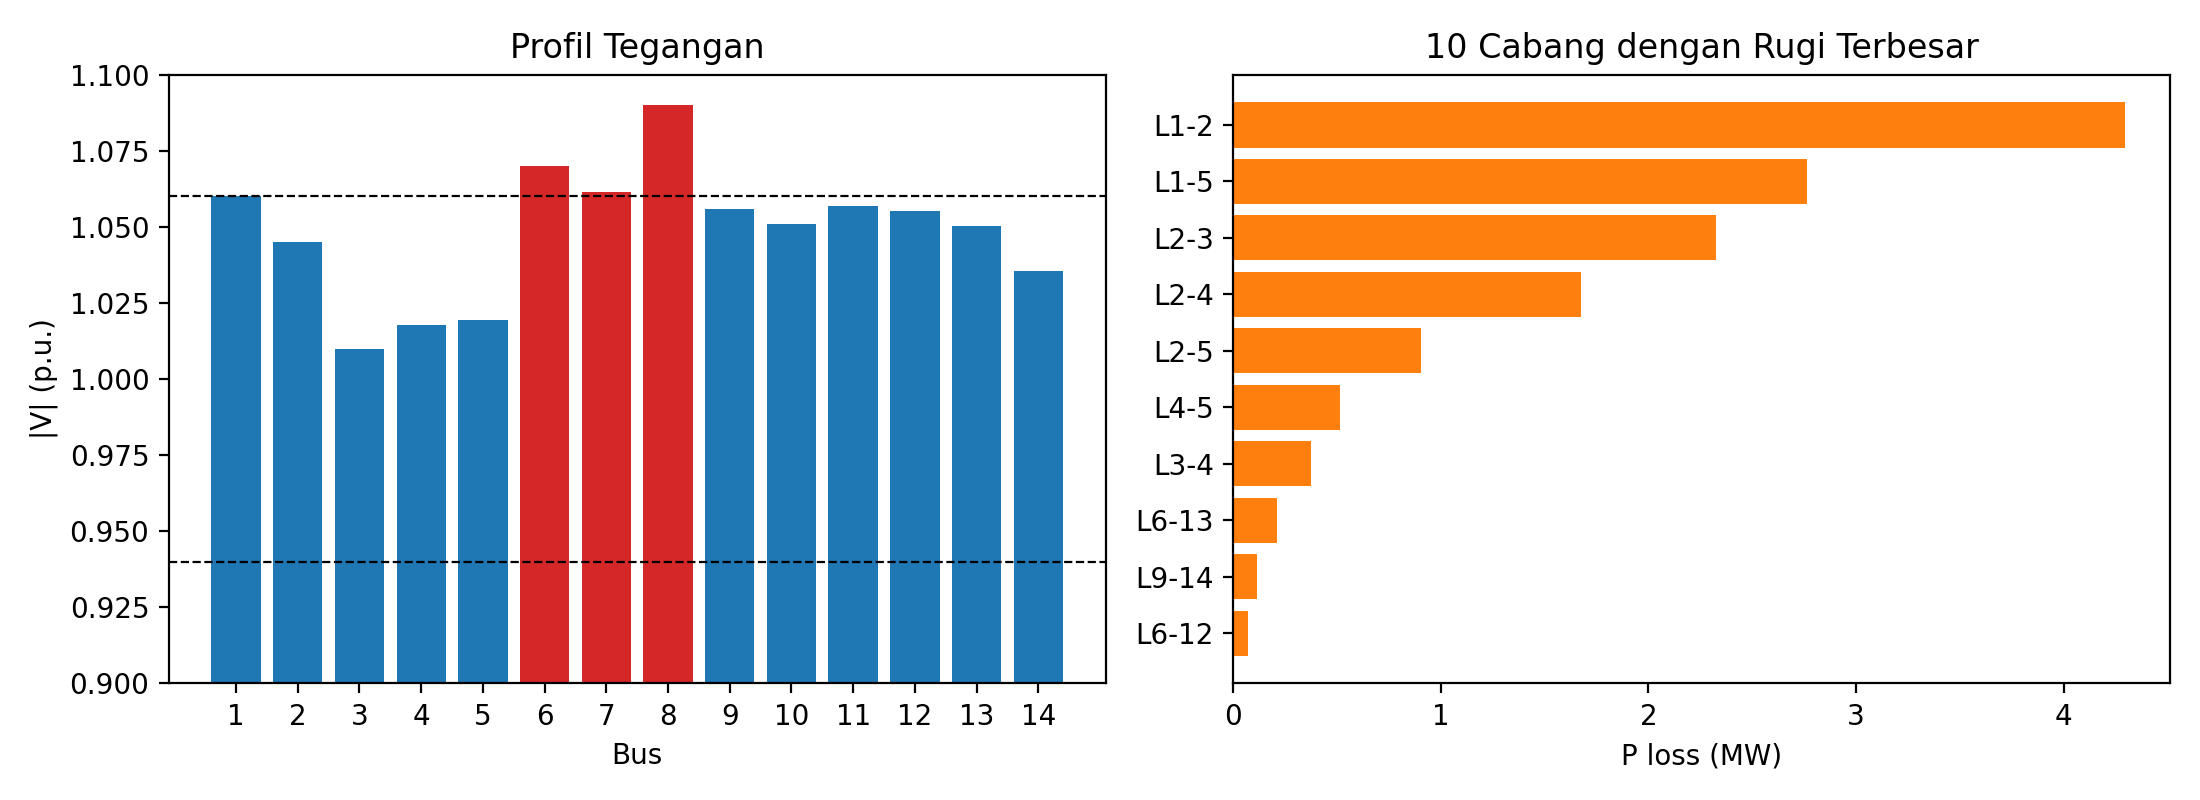
\includegraphics[width=0.95\textwidth]{../figures/profil_tegangan_rugi.png}
  \caption{Profil tegangan 14 bus dan distribusi 10 cabang penyumbang rugi aktif terbesar pada kondisi dasar IEEE 14-Bus (rugi total $13{,}393\text{ MW}$ atau $5{,}17\%$ dari beban $259{,}0\text{ MW}$).}
\end{figure}

\begin{checkpointbox}[Titik Periksa Mandiri Modul 3]
Validasi silang terhadap solver Modul 2 menghasilkan deviasi maksimum $\max ||V_{\text{scratch}}| - |V_{\text{pp}}|| = \mathbf{4{,}44\times 10^{-16}\text{ p.u.}}$. Tiga penyumbang rugi daya aktif terbesar adalah \texttt{L1-2} ($4{,}298\text{ MW}$), \texttt{L1-5} ($2{,}763\text{ MW}$), dan \texttt{L2-3} ($2{,}323\text{ MW}$).
\end{checkpointbox}

% ==================== BAB 5: MODUL 4 ====================
\chapter{Modul 4: Kontinjensi $N-1$ \& Proyek Capstone}

\section{Kriteria Keamanan $N-1$ \& Indeks Keparahan ($PI$)}
Sistem aman $N-1$ apabila untuk setiap pelepasan satu saluran atau transformator terpenuhi $0{,}95 \le |V_i| \le 1{,}10\text{ p.u.}$, $\text{loading}_l \le 100\%$, tanpa pemutusan beban maupun \textit{islanding}. Indeks keparahan gabungan dihitung dengan eksponen penalti $2n = 4$:
\begin{equation}
  PI_k = \sum_{l=1}^{N_{\text{br}}} \frac{w_l}{2n}\left(\frac{|S_l|}{S_l^{\text{rated}}}\right)^{2n}
       + \sum_{i=1}^{N_b} \frac{w_{v,i}}{2n}\left(\frac{|V_i| - V_i^{\text{nom}}}{\Delta V_i^{\text{lim}}}\right)^{2n}
\end{equation}

\begin{table}[H]
\centering
\caption{Peringkat 8 Kontinjensi $N-1$ Terparah + Kasus \textit{Islanding} pada IEEE 14-Bus}
\small
\begin{tabular}{@{}clcccccc@{}}
\toprule
\textbf{Rank} & \textbf{Kontinjensi} & \textbf{Status} & \textbf{Load Maks (\%)} & \textbf{Terberat} & \textbf{\# Over} & \textbf{$|V|_{\min}$ (p.u.)} & \textbf{$PI$} \\
\midrule
1 & \texttt{L2-3} & OK & 301,48 & \texttt{L3-4} & 4 & 1,0100 & 95,50 \\
2 & \texttt{L1-2} & OK & 251,16 & \texttt{L1-5} & 3 & 0,9935 & 60,05 \\
3 & \texttt{T5-6} & OK & 143,85 & \texttt{L7-9} & 7 & 1,0100 & 27,04 \\
4 & \texttt{L1-5} & OK & 129,99 & \texttt{L2-5} & 3 & 1,0064 & 12,84 \\
5 & \texttt{L2-4} & OK & 111,57 & \texttt{L2-5} & 2 & 1,0071 & 10,94 \\
6 & \texttt{T4-7} & OK & 124,91 & \texttt{T4-9} & 1 & 1,0100 & 10,87 \\
7 & \texttt{L7-9} & OK & 121,25 & \texttt{T4-9} & 1 & 1,0100 & 10,11 \\
8 & \texttt{L4-5} & OK & 111,58 & \texttt{L2-4} & 1 & 1,0100 & 9,69 \\
\midrule
--- & \texttt{L7-8} & \textbf{ISLANDING} & 73,69 & \texttt{L1-2} & 0 & Bus 8 terisolasi & 4,98 \\
\bottomrule
\end{tabular}
\end{table}

\begin{figure}[H]
  \centering
  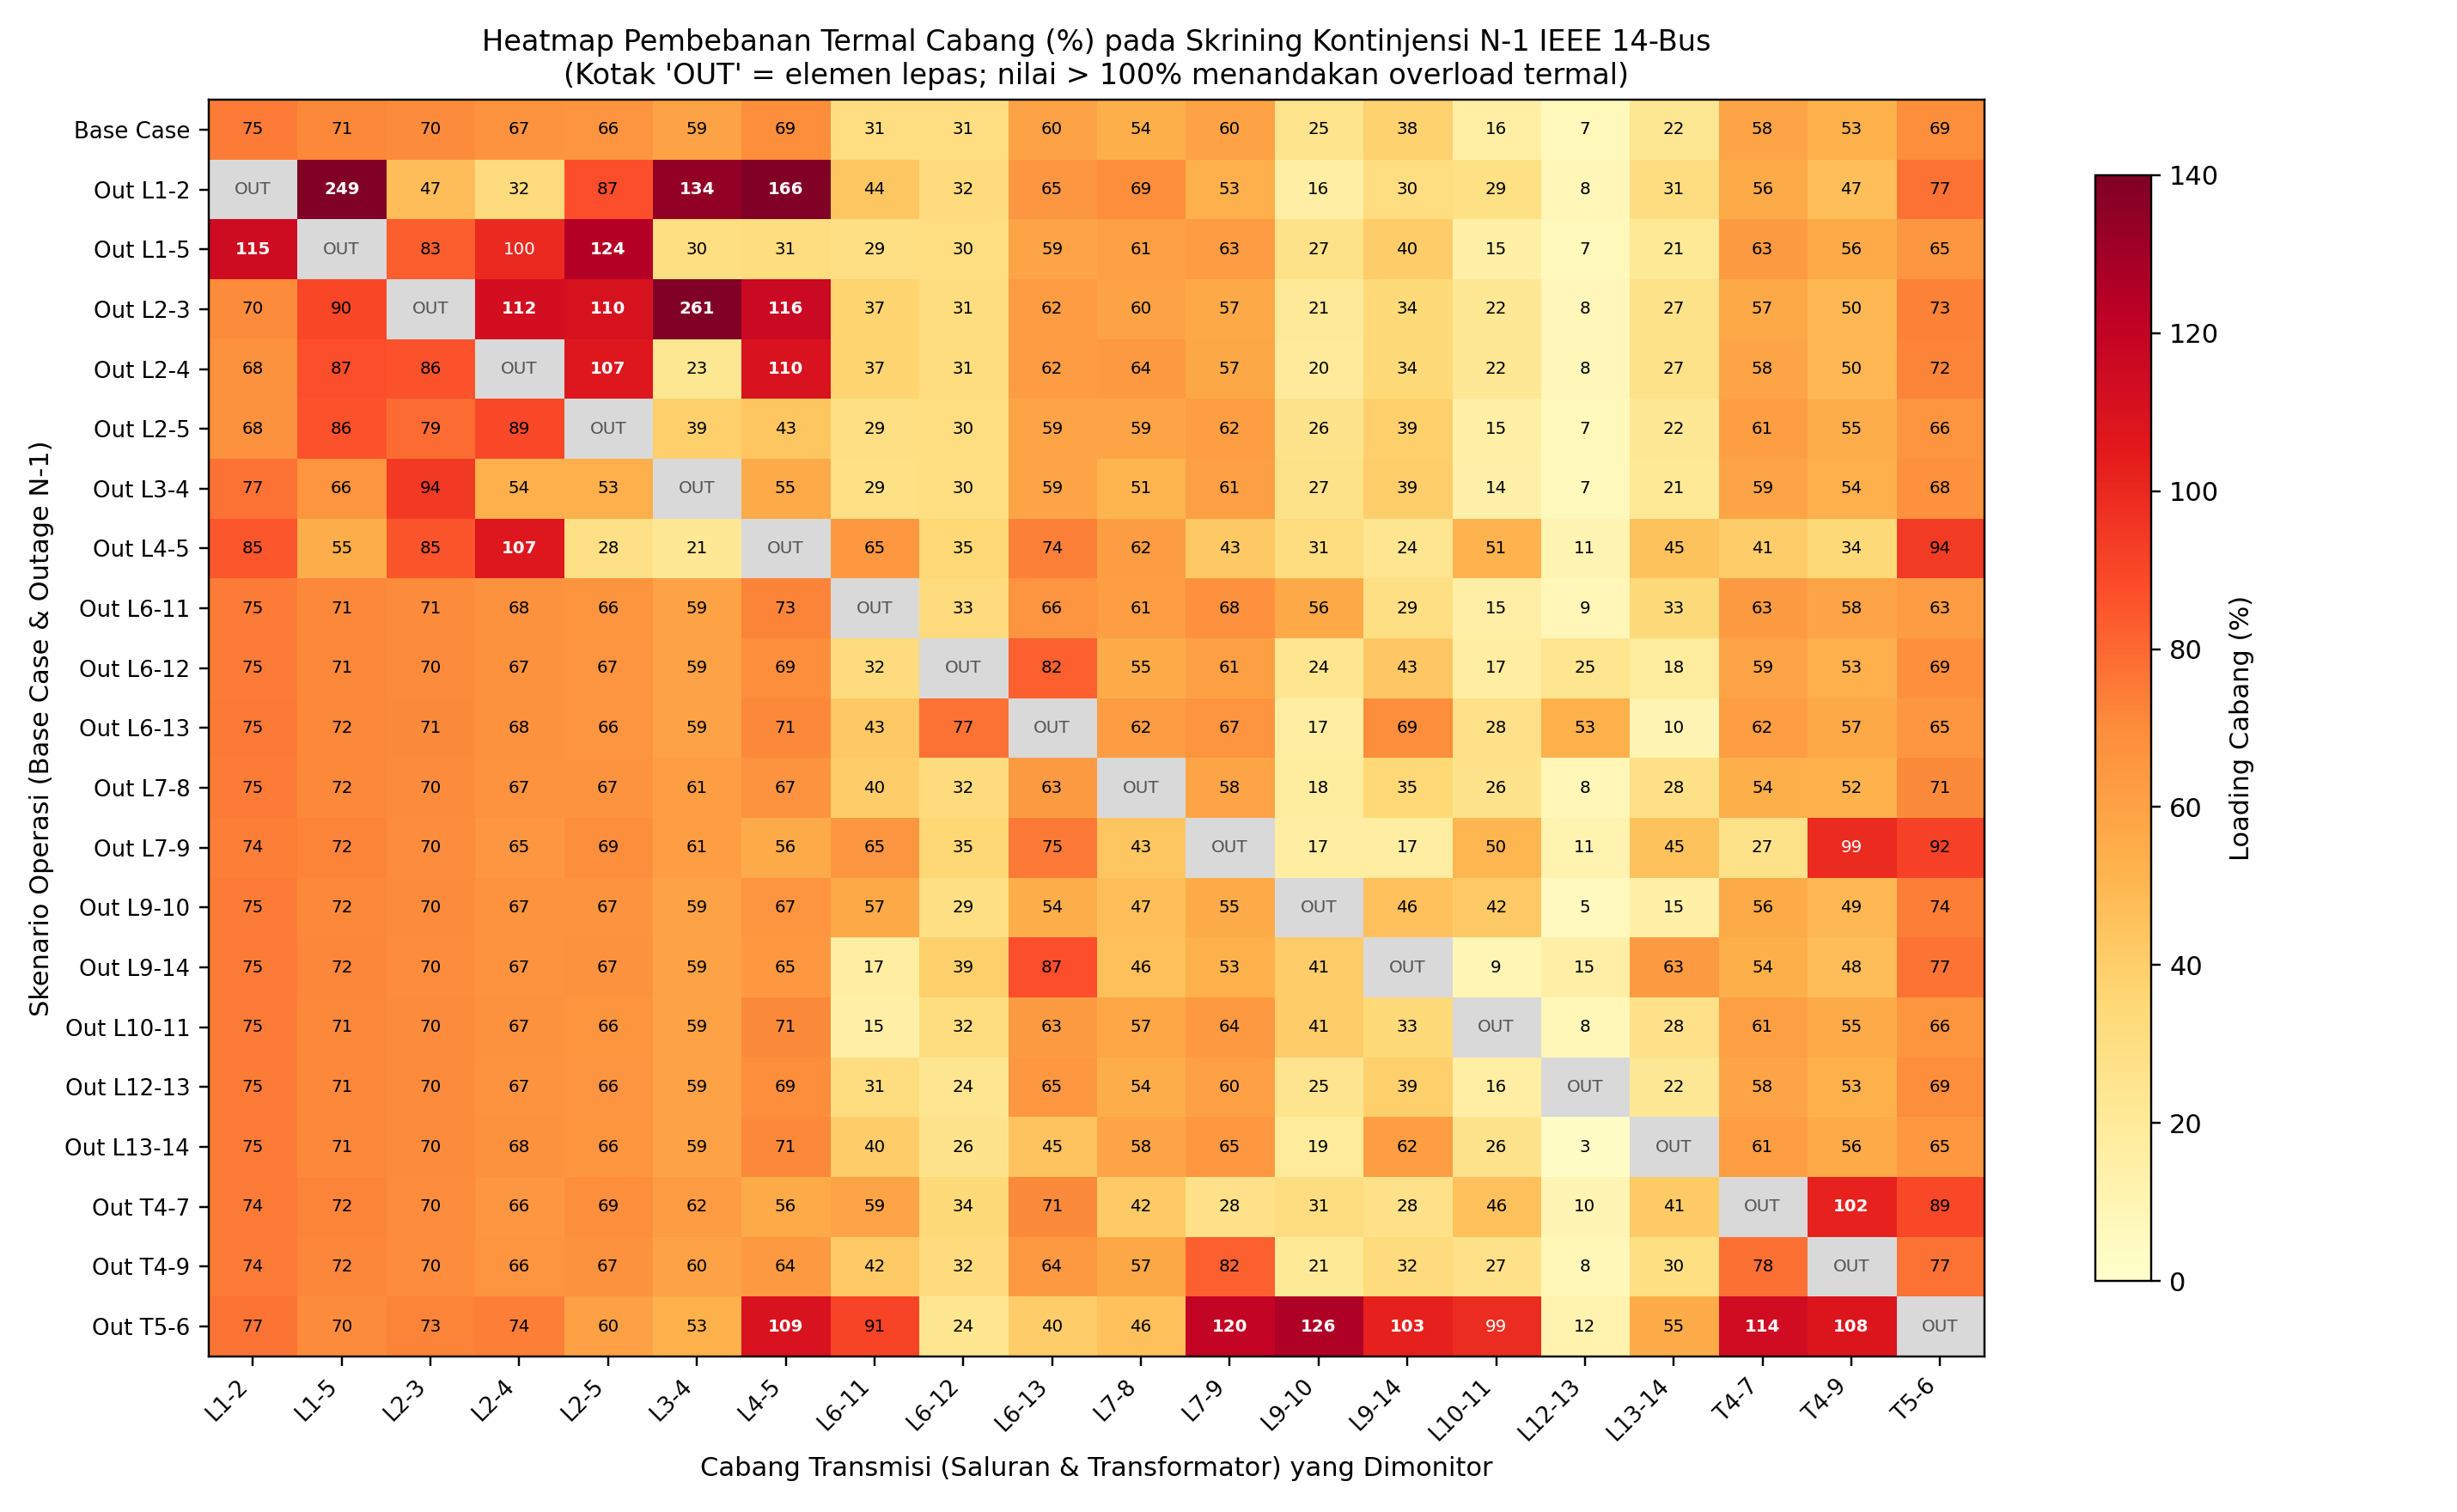
\includegraphics[width=0.92\textwidth]{../figures/n1_line_loading_heatmap.png}
  \caption{Heatmap matriks pembebanan arus cabang ($21 \times 20$) untuk seluruh kontinjensi tunggal pada IEEE 14-Bus (\texttt{pandapower\_workflow.py}).}
\end{figure}

\begin{figure}[H]
  \centering
  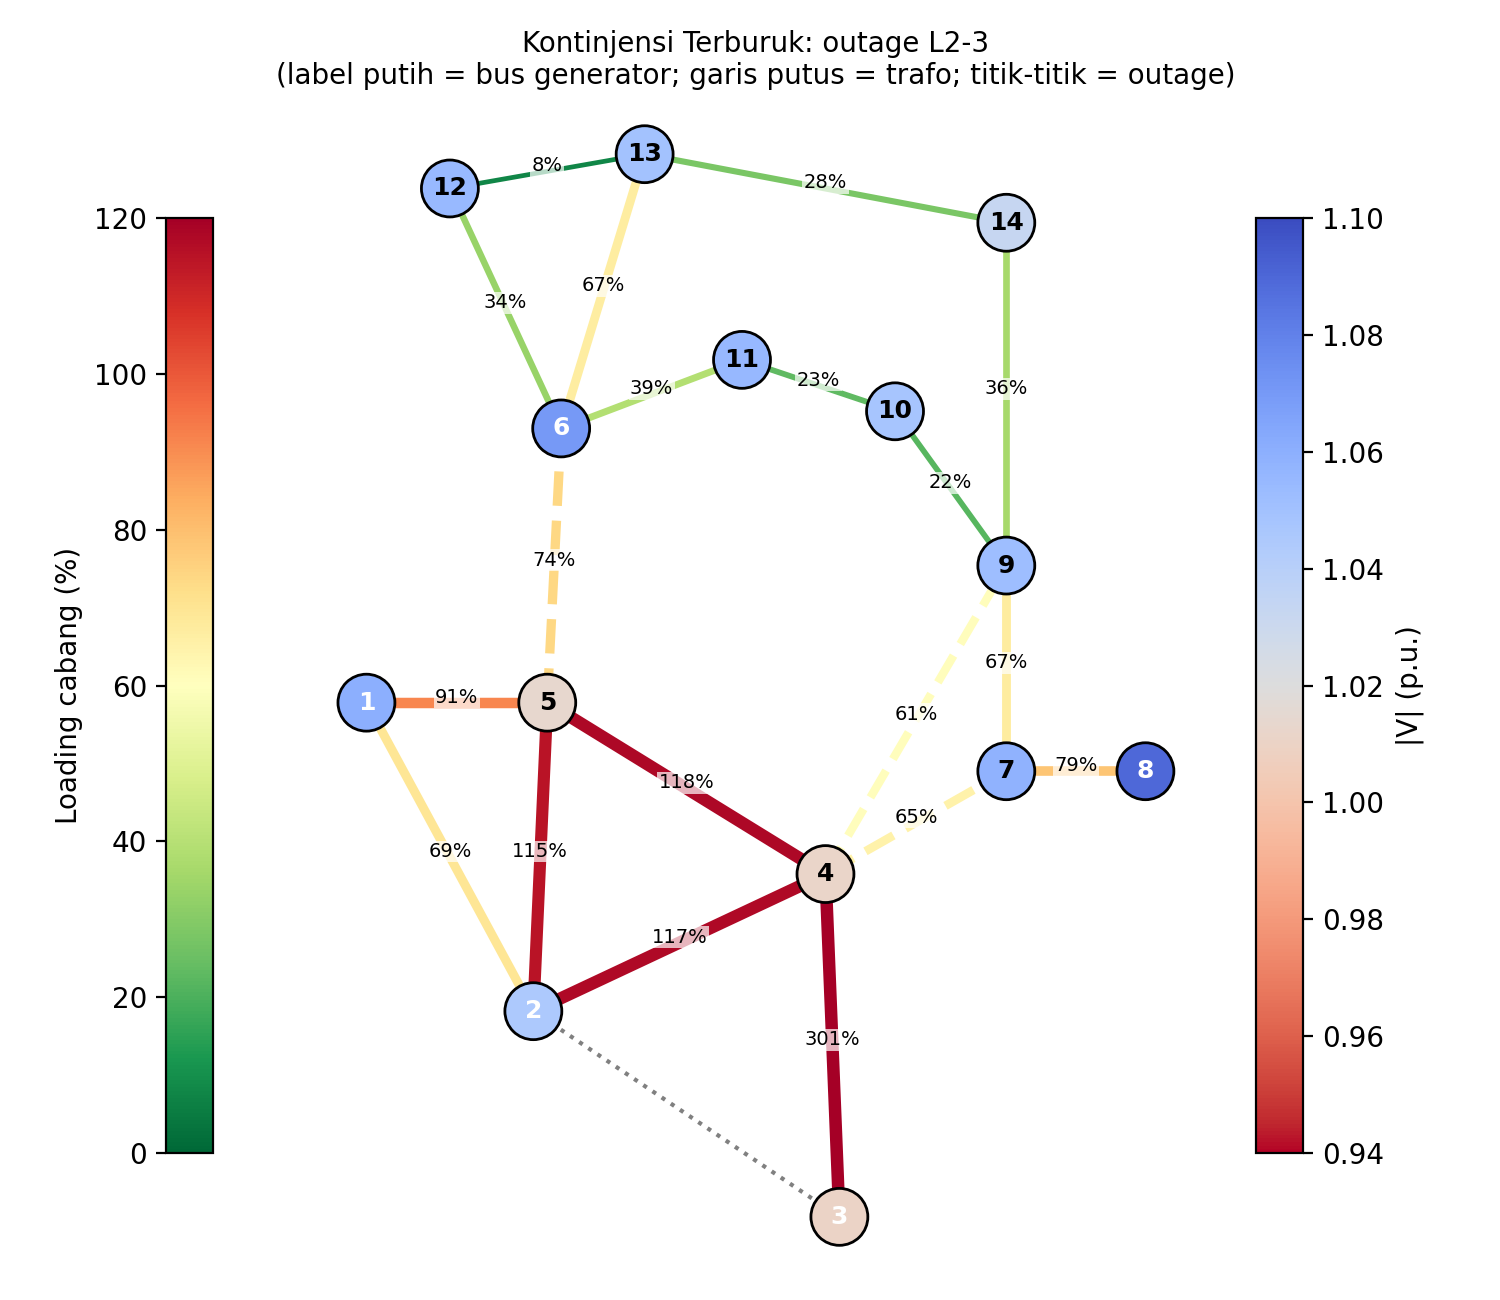
\includegraphics[width=0.68\textwidth]{../figures/topologi_kontinjensi_terburuk.png}
  \caption{Diagram topologi kontinjensi terburuk (pelepasan saluran \texttt{L2-3}) yang menyoroti 4 saluran mengalami \textit{overload} termal berat.}
\end{figure}

\section{Skema Penilaian Akhir \& Proyek Capstone}
Bobot evaluasi pelatihan: Modul 1 (15\%), Modul 2 (25\%), Modul 3 (20\%), Modul 4 (25\%), dan Proyek Capstone (15\%). Peserta memilih salah satu jalur Capstone: (A) Studi $N-1$ IEEE 30-Bus, (B) Profil kecepatan solver pada sistem $>1.000$ bus, (C) Integrasi PLTS/PLTB, atau (D) Kontinjensi berbasis risiko.

% ==================== BAB 6: SERI LANJUTAN LEVEL 2 ====================
\chapter{Seri Lanjutan Level 2: AC-OPF, PV Hosting Capacity \& Risiko $N-2$}

Bab ini merangkum modul kurikulum \textbf{Seri Lanjutan Level 2 (24 JP / 3 Hari)} beserta hasil komputasi eksak yang dapat direproduksi melalui skrip \texttt{level2/level2\_advanced\_studies.py}.

\section{Modul L2-1: Optimal Power Flow (AC-OPF \& LMP)}
AC-OPF meminimalkan total biaya pembangkitan kuadratik $C(P_g) = c_{2,g}P_g^2 + c_{1,g}P_g + c_{0,g}$ terhadap kendala aliran daya AC, koridor tegangan $[0{,}95;\; 1{,}06]\text{ p.u.}$, dan batas termal cabang $\le 100\%$:
\begin{itemize}[leftmargin=1.5em]
  \item Biaya operasi turun dari $\$8.170{,}15/\text{jam}$ menjadi \textbf{$\$8.082{,}26/\text{jam}$} (hemat $1{,}08\%$).
  \item Rugi daya aktif turun tajam dari $13{,}393\text{ MW}$ menjadi \textbf{$9{,}466\text{ MW}$} (reduksi \textbf{$29{,}3\%$}) melalui redistribusi pembangkitan Bus 1 ($196{,}70\text{ MW}$), Bus 2 ($37{,}14\text{ MW}$), dan Bus 3 ($34{,}49\text{ MW}$).
  \item Harga marjinal lokasional (\textit{Locational Marginal Price / LMP}) berada pada rentang \textbf{$\$36{,}92\text{--}\$41{,}52/\text{MWh}$}.
\end{itemize}

\begin{figure}[H]
  \centering
  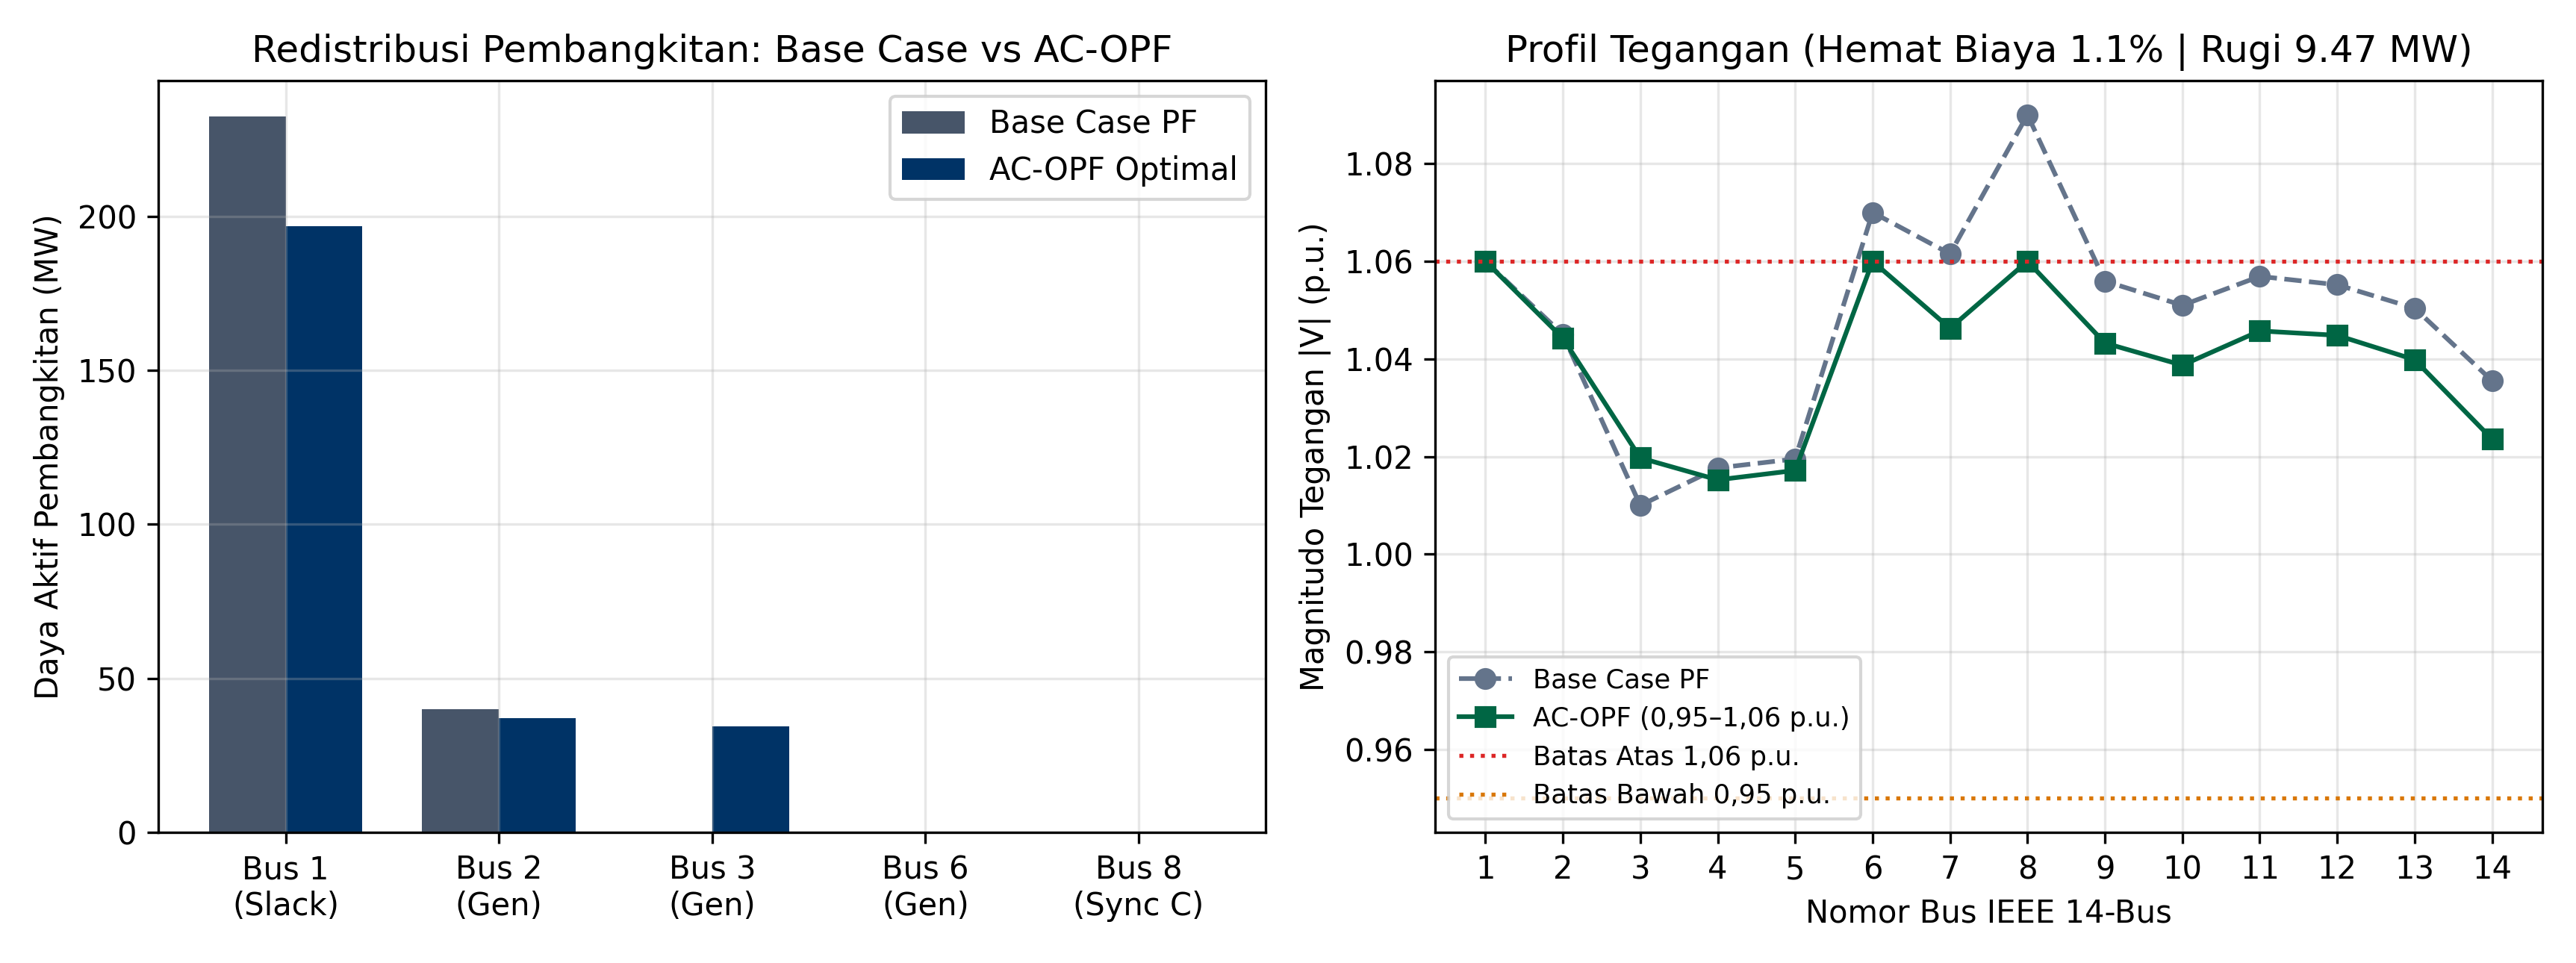
\includegraphics[width=0.95\textwidth]{../figures/level2_opf_comparison.png}
  \caption{Perbandingan redistribusi pembangkitan aktif dan profil tegangan antara kondisi dasar (Base Case PF) dan solusi AC-OPF pada IEEE 14-Bus.}
\end{figure}

\section{Modul L2-2: Studi \textit{PV Hosting Capacity}}
Sapuan injeksi PLTS (\texttt{pp.create\_sgen}, $\cos\varphi = 1$) pada bus beban subsistem (Bus 10, 13, dan 14) dengan batas tegangan area beban $\le 1{,}06\text{ p.u.}$ menghasilkan kapasitas hosting:
\begin{itemize}[leftmargin=1.5em]
  \item \textbf{Bus 10:} $10{,}0\text{ MW}$ (terbatas oleh kedekatan terhadap Bus 11 yang bertegangan dasar tinggi $1{,}0569\text{ p.u.}$).
  \item \textbf{Bus 13:} $20{,}0\text{ MW}$ dan \textbf{Bus 14:} $25{,}0\text{ MW}$ (memiliki \textit{headroom} tegangan terbesar karena tegangan awal $1{,}0355\text{ p.u.}$).
\end{itemize}

\begin{figure}[H]
  \centering
  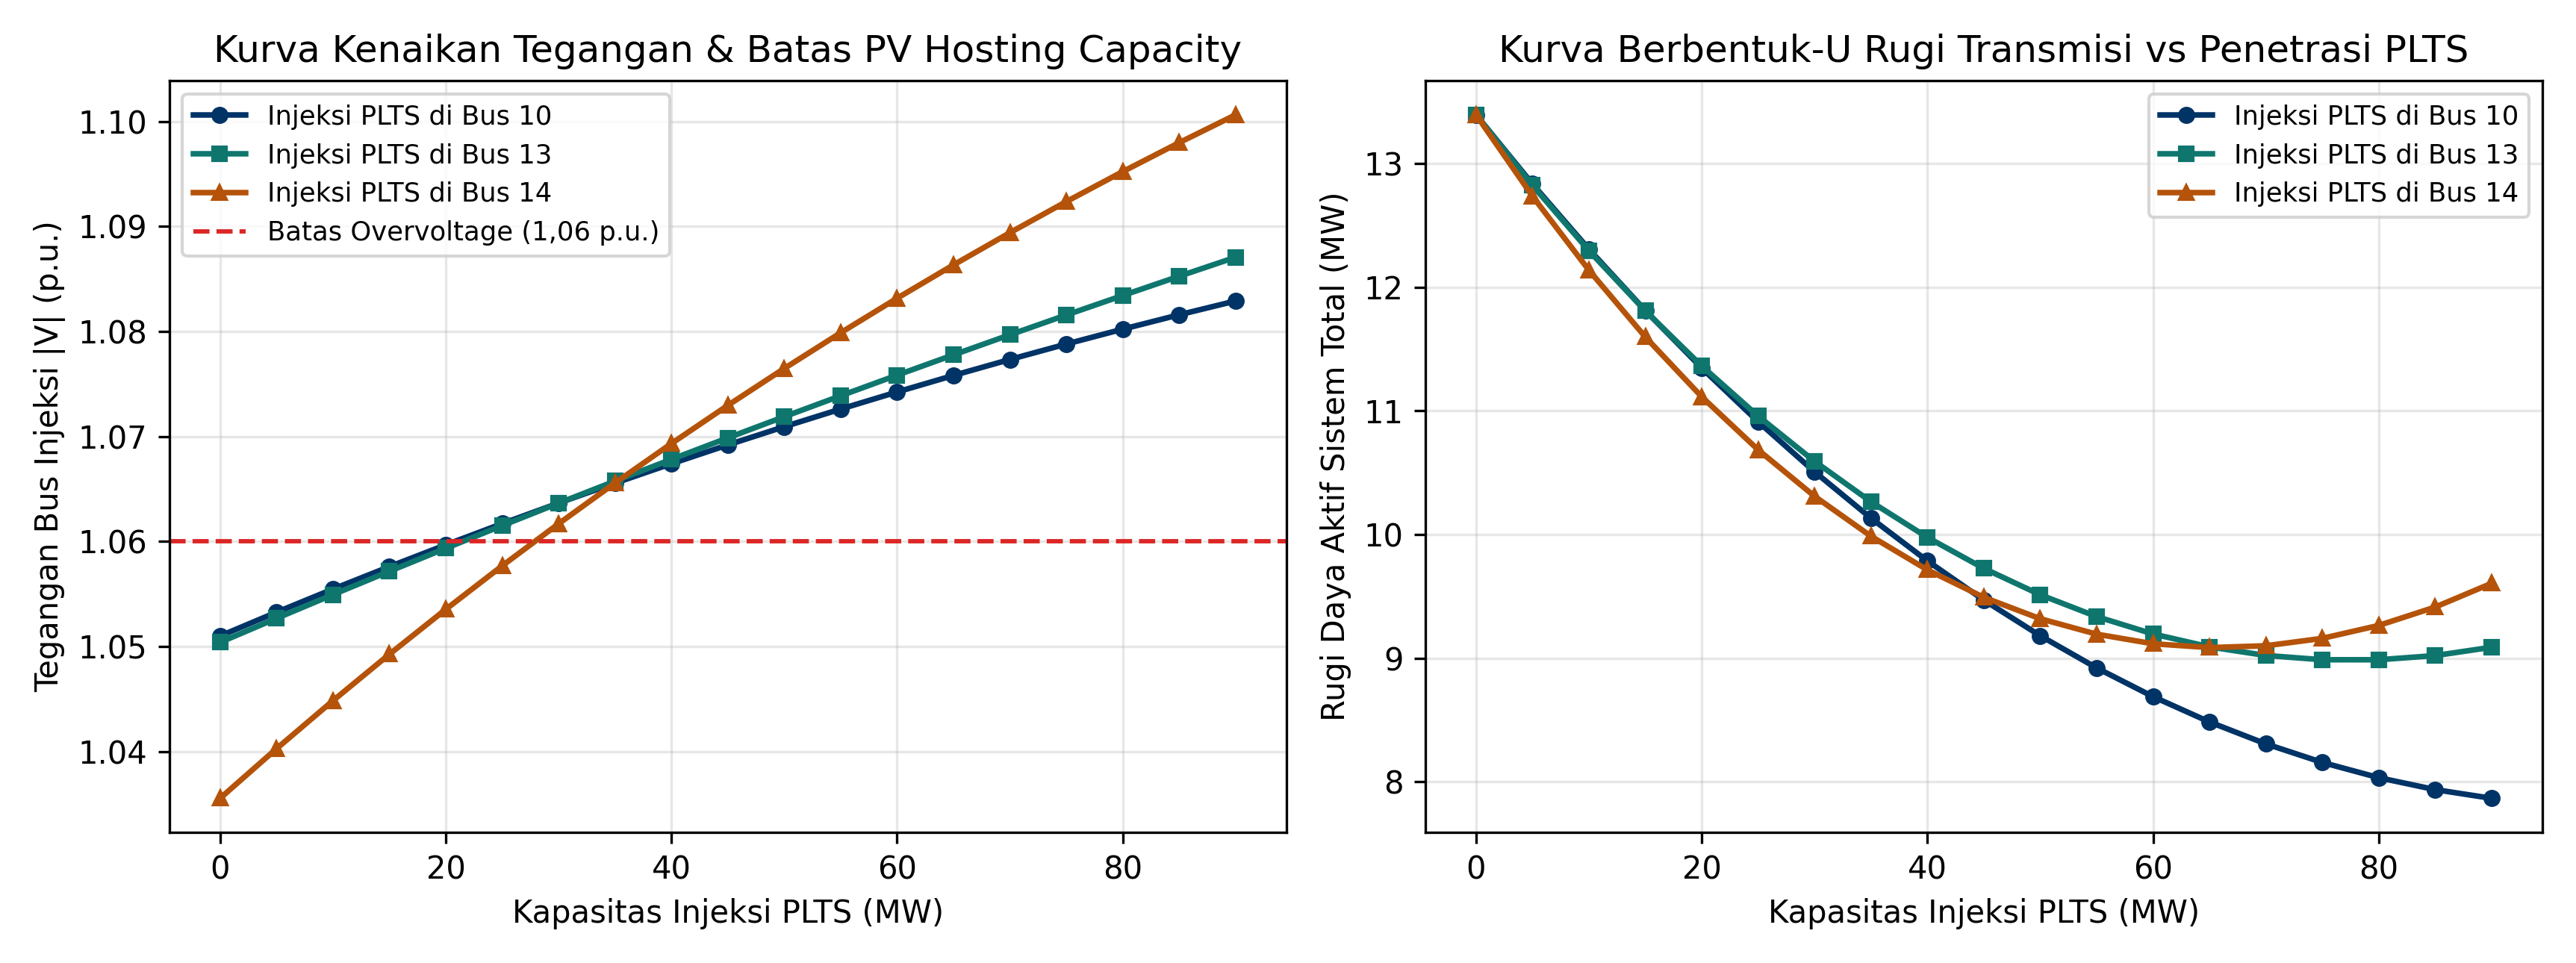
\includegraphics[width=0.95\textwidth]{../figures/level2_pv_hosting_capacity.png}
  \caption{Kurva kenaikan tegangan dan pola berbentuk-U rugi daya aktif sistem terhadap peningkatan penetrasi PLTS pada Bus 10, 13, dan 14.}
\end{figure}

\section{Modul L2-3: Skrining Kontinjensi Ganda ($N-2$) Berbasis Risiko}
Pada IEEE 14-Bus terdapat $\binom{20}{2} = 190$ pasangan kontinjensi ganda. Dengan probabilitas gangguan simultan $p_{ij} = p_i p_j$, Indeks Risiko dirumuskan sebagai:
\begin{equation}
  RI_{ij} = p_i p_j \cdot \left(PI_{S,ij} + PI_{V,ij} + 250\,N_{\text{bus,terisolasi}}\right)
\end{equation}
Evaluasi otomatis seluruh 190 pasangan mendeteksi \textbf{27 skenario \textit{islanding}}, dengan peringkat risiko teratas: (1) \texttt{L1-2 + L1-5} ($13$ bus terisolasi dari Slack, $RI\times 10^3 = 119{,}35$), (2) \texttt{L9-14 + L13-14} (Bus 14 terisolasi, $RI\times 10^3 = 30{,}82$), dan (3) \texttt{L6-12 + L12-13} (Bus 12 terisolasi, $RI\times 10^3 = 22{,}83$).

\begin{figure}[H]
  \centering
  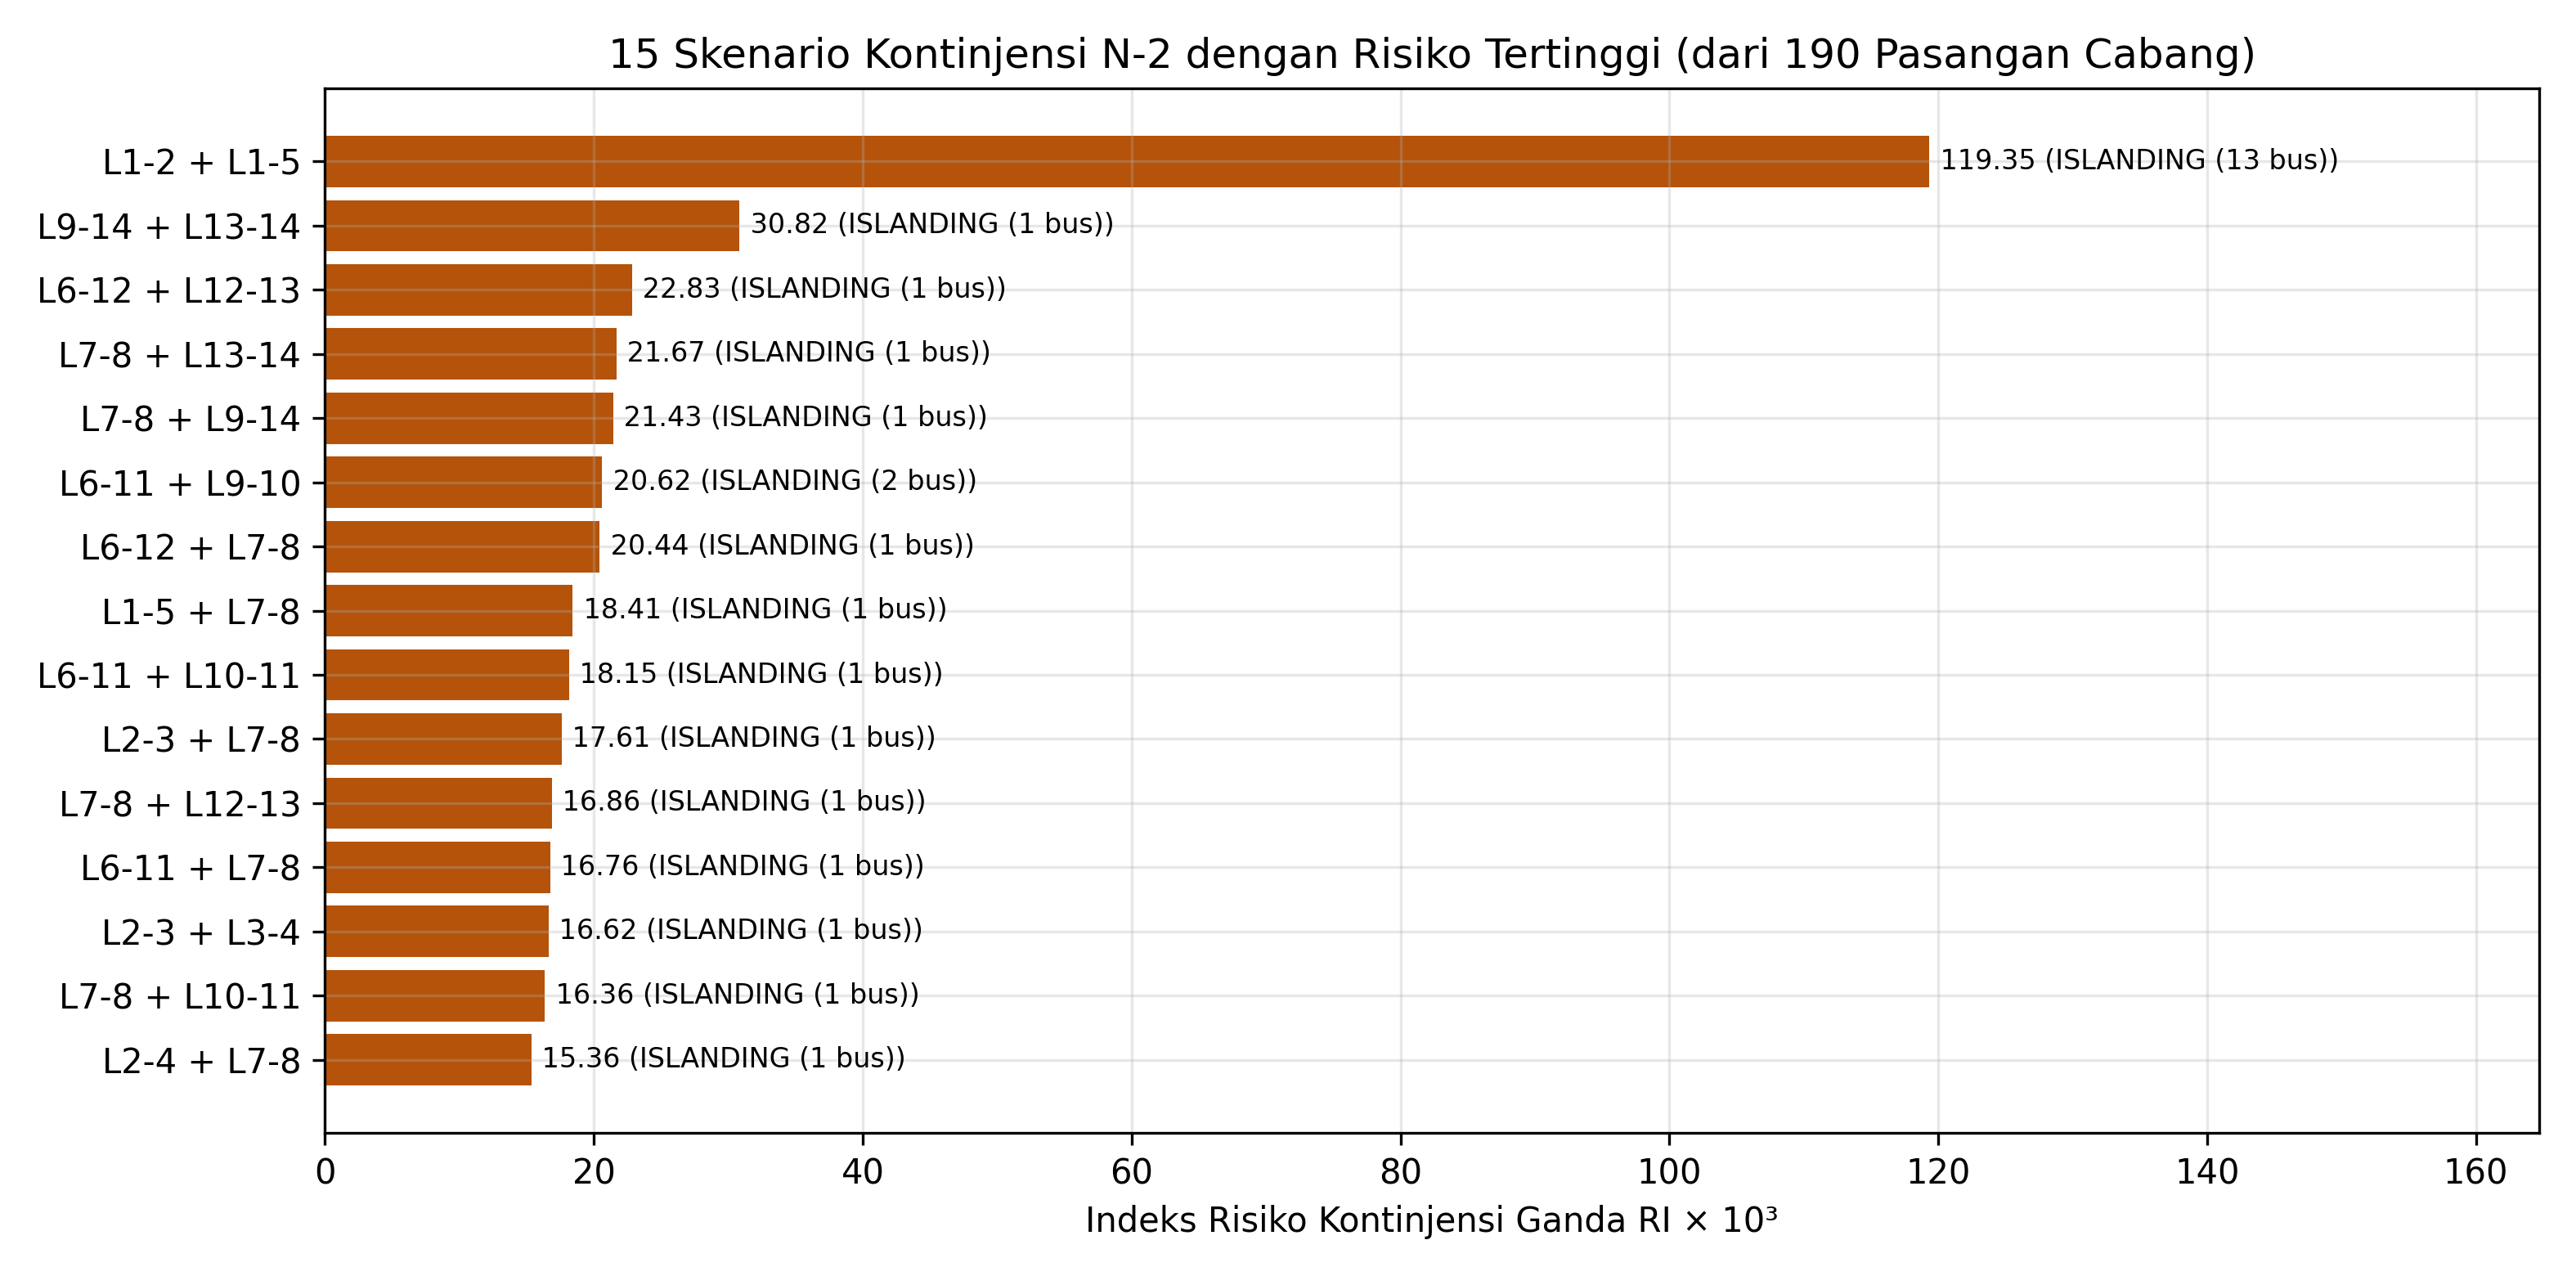
\includegraphics[width=0.92\textwidth]{../figures/level2_n2_risk_top15.png}
  \caption{15 skenario kontinjensi ganda ($N-2$) dengan Indeks Risiko tertinggi dari 190 pasangan cabang IEEE 14-Bus (\texttt{level2/hasil/n2\_risk\_ranking.csv}).}
\end{figure}

% ==================== LAMPIRAN ====================
\appendix
\chapter{Panduan \textit{Troubleshooting}, Kuis C1--C6 \& Referensi}

\section{Matriks \textit{Troubleshooting} Konvergensi}
\begin{table}[H]
\centering
\small
\begin{tabular}{@{}p{3.6cm}p{4.8cm}p{5.4cm}@{}}
\toprule
\textbf{Gejala} & \textbf{Kemungkinan Penyebab} & \textbf{Tindakan Korektif} \\
\midrule
NR berosilasi / divergen & Tanda/indeks Jacobian keliru & Uji beda hingga terpusat ($\varepsilon = 10^{-7}$) \\
Konvergen $> 6$ iterasi & Turunan diagonal $H_{ii}, L_{ii}$ salah & Cocokkan kembali dengan Tabel 3.1 \\
\texttt{MatrixRankWarning} & Bus terisolasi / pulau tanpa Slack & Jalankan deteksi topologi graf \\
FDLF lambat / gagal & Rasio $R/X$ saluran tinggi & Beralih ke NR penuh atau skema BX \\
\bottomrule
\end{tabular}
\end{table}

\section{Contoh Kuis Formatif Berjenjang (Bloom C1--C6)}
\begin{enumerate}[leftmargin=1.5em]
  \item \textbf{[C1]} Sebutkan besaran yang diketahui dan dicari pada bus PV.
  \item \textbf{[C2]} Mengapa $Y_{\text{bus}}$ menjadi tidak simetris saat terdapat transformator \textit{phase-shifter}?
  \item \textbf{[C3]} Hitung elemen $Y_{12}$ untuk saluran $z = 0{,}02 + j0{,}06\text{ p.u.}$ dengan tap $t = 0{,}98$ di sisi bus 1.
  \item \textbf{[C4]} Buktikan konvergensi kuadratik dari riwayat mismatch NR IEEE 14-Bus.
  \item \textbf{[C5]} Pilih solver terbaik untuk skrining 5.000 kontinjensi setiap 5 menit dan jelaskan risikonya.
  \item \textbf{[C6]} Rancang skema mitigasi untuk pelepasan \texttt{L2-3} serta strategi peningkatan \textit{PV hosting capacity} di Bus 10.
\end{enumerate}

\section{Referensi Utama}
\begin{enumerate}[leftmargin=1.5em]
  \item Grainger, J. J., \& Stevenson, W. D. \textit{Power System Analysis}. McGraw-Hill.
  \item Glover, J. D., Overbye, T. J., \& Sarma, M. S. \textit{Power System Analysis and Design}. Cengage.
  \item Stott, B., \& Alsa\c{c}, O. (1974). Fast Decoupled Load Flow. \textit{IEEE Trans. PAS}, 93(3), 859--869.
  \item Zimmerman, R. D., Murillo-S\'anchez, C. E., \& Thomas, R. J. (2011). MATPOWER. \textit{IEEE Trans. Power Systems}, 26(1).
  \item Thurner, L., et al. (2018). pandapower --- An Open-Source Python Tool for Convenient Modeling, Analysis, and Optimization of Electric Power Systems. \textit{IEEE Trans. Power Systems}, 33(6).
  \item Wood, A. J., Wollenberg, B. F., \& Shebl\'e, G. B. \textit{Power Generation, Operation, and Control}. Wiley.
\end{enumerate}

\end{document}
